% !TeX spellcheck = en_GB

\section{Monitor Pipeline}
\label{sec:concept:pipeline}

\begin{itemize}
	\item goal == monitor KNX traffic
	\item notion of \emph{project} is used to differentiate unique, not comparable KNX networks. Can be seen as a common prefix for everything which need to be named internally.
	\item monitoring should include the whole network/world view
	\item monitoring needs to be distributed, so Line Couplers can be configured properly
	\item monitoring is done by agents
	\item agents will send data gather over a time window to the collector (ref to neflow terminology)
	\item time windows of agents are synchronised (by the collector) to make data analysis more reliable
	\item agents send gathered data to collector via KNX network
	\item collector stores windows immediately in InfluxDB
	\item collector checks regularly the InfluxDB, if all agents send in their time window
	\item if so the collector relays all windows, describing the same time slot (+/- a couple seconds), to the analyser modules
	\item if not all windows are in by specified timeout (10s or so) they are relayed anyway
	\item bundled windows are distributed by pub-sub-server independently to different analytical modules
	\item analytical modules compare the windows to a base-line model (in different fashions)
\end{itemize}

\begin{figure}[h]
	\centering
	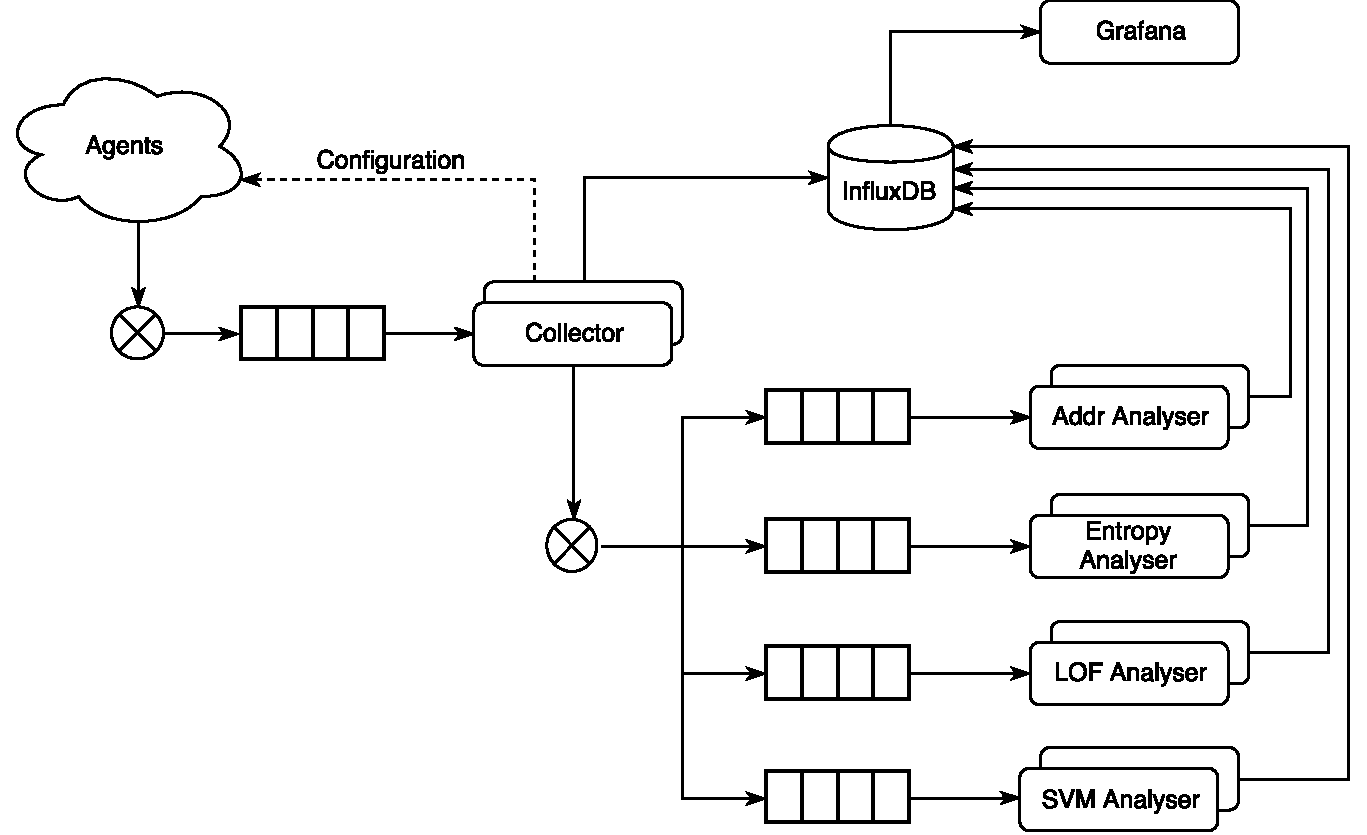
\includegraphics[width=\textwidth]{figures/300-concept-architecture.pdf}
	\caption[Pipeline Architecture]{Architecture of the monitoring pipeline}
	\label{fig:concept:architecture}
\end{figure}

\section{Design of Netflow Agent}
\label{sec:concept:agent}
cf. \textcite{Bloedorn2001} for a basic "How to get started" IDS Data Mining Infrastructure
\subsection{Truncating and Statistic Gathering}

\section{The Collector Module}
\label{sec:concept:collector}

\begin{itemize}
	\item responsible for
		\subitem collecting data from agents through the KNX network
		\subitem storing raw time windows in InfluxDB
		\subitem relaying raw, synchronised time windows to analytical modules
	\item listens to a single message queue containing time windows from all agents assigned to the same project
	\item agents must have unique names within one project
	\item windows are parsed and then submitted into the InfluxDB, tagged with the agent-name and the project
	\item window is split into different measurements (tables) determined by the KNX fields observed.
	\item one additional measurement (table) \code{agent-status}, representing general status information
		\subitem timely length of the window
		\subitem end timestamp of the window
		\subitem boolean if window was relayed or not
	\item collector regularly checks the InfluxDB for unrelayed windows (latest ones first)
	\item windows are grouped by time slot
	\item if all agents have submitted a window for a specific timeslot these windows are bundled and relayed to the analyser message exchange (cf.~Figure~\ref{fig:concept:architecture})
	\item for all successfully relayed windows set the \code{realayed} flag in the \code{agent-status} measurement to \code{true}
\end{itemize}

\section{Analyser Modules}
\label{sec:concept:anal}

\subsection{The Address Analyser}
\label{sec:concept:anal:addr}

\subsection{The Local Outlier Factor Analyser}
\label{sec:concept:anal:lof}

\subsection{The Entropy Analyser}
\label{sec:concept:anal:entropy}

\section{Possible Errors and Design Drawbacks}
\label{sec:concept:flaws}
\begin{itemize}
	\item Errors in handling daylight saving time and time zones, due to missing time zone information in log
		\subitem simulated agent might be a bit off
		\subitem gap plus cummulated packets when daylight saving changes
\end{itemize}
